\chapter{Логическое моделирование вариантов принятия решения по рациональному использованию лесных ресурсов}

\def\textsubscript#1{{\tiny{}#1}}

Содержание данной главы базируется на \cite{dissche} и \cite{dissAsya}, проводится обобщение результатов, представленных в данных диссертациях. Указанное обобщение базируется на применении алгоритмов и подпрограмм, представленных в этих работах, в качестве подпрограмм в решении задачи логического прогнозирования следствий принятия некоторого решения по управлению лесными ресурсами промышленного региона.


\section*{Введение}
Российская Федерация обладает большими запасами лесных ресурсов (ЛР), которые размещены неравномерно, местами истощены, а значительная часть территории страны относится к особо охраняемым территориям, где ведение хозяйственной деятельности ограничено. Значительная часть сибирских и дальневосточных регионов РФ  являются источником лесных ресурсов, которые составляют основную экспортную составляющую для этих регионов.

Проблема формирования политики использования ЛР является чрезвычайно важной задачей для лиц, принимающих решения (ЛПР) в управлении лесопромышленным регионом. ЛПР  в процессе принятия решения сталкивается с задачами, которые являются «антиинтуитивными». Под «антиинтуитивными» решениями понимаются решения, которые не являются «очевидно хорошими» на взгляд эксперта, т.е. решения, которые требуют специального исследования. Эффективность принимаемых ЛПР решений в первую очередь зависит от объема, вида и качества исходных данных о состоянии ЛР, а также прогнозов развития ЛР в зависимости от принимаемых ЛПР решений (политики заготовки ЛР).

На процесс принятия решения часто воздействуют различные случайные параметры, усложняющие процедуру принятия решения. Недостаток информации об их распределении (сложность их измерения) приводит к необходимости принятия гипотез как об области  изменения данных параметров, так и о характере их распределения (о функции распределения вероятностей). Правильность используемых гипотез необходимо проверять с помощью методов оценки статистических гипотез. Проблемы принятия решений с недетерминированными параметрами называют проблемами принятия решений в условиях недостатка информации. Чем меньше информации об исследуемом объекте есть, тем больше может оказаться различие между ожидаемым и действительным результатами принимаемых решений в целом [41].

Современные системы поддержки принятия решения (СППР), возникшие как естественное развитие и продолжение управленческих информационных систем и систем управления базами данных, представляют собой системы, максимально приспособленные к решению задач повседневной управленческой деятельности, и являются инструментом, призванным оказать помощь ЛПР. С помощью СППР могут решаться неструктурированные и слабоструктурированные многокритериальные задачи.

СППР, как правило, являются результатом мультидисциплинарного исследования, включающего теории баз данных, искусственного интеллекта [53, 72], интерактивных компьютерных систем [73], методов имитационного моделирования [54, 76].

Ранние определения СППР (в начале 70-х годов ХХ века) отражали следующие три момента:
\begin{enumerate}
\item возможность оперировать с неструктурированными или слабоструктурированными задачами, в отличие от задач, с которыми имеет дело исследование операций;
\item интерактивные автоматизированные, т.е. реализованные на базе компьютера, системы;
\item разделение данных и моделей.
\end{enumerate}

В данной главе под СППР понимется интерактивная автоматизированная система, которая помогает ЛПР использовать имеющиеся данные и математические модели для идентификации и решения поставленных перед ним задач и принятия управленческих и других решений.

СППР являются человеко-машинными программными объектами, которые позволяют ЛПР использовать разнообразные методы (данные, знания, объективные и субъективные модели) для анализа и решения слабоструктурированных и неструктурированных задач. Идея СППР возникла как попытка автоматизации естественных человеческих действий по анализу имеющейся информации, планированию действий и т.п. с целью решения конкретной поставленной задачи.

Основной частью СППР является генератор решений (рис. 1.1), который действует на основании исходных данных (блок «Данные») об объекте исследования и описания постановки задачи. В процессе принятия решения генератор решений взаимодействует с подсистемой искусственного интеллекта, которая, в свою очередь, использует базу знаний для построения базовой структуры модели объекта исследования по известным исходным данным [18]. Также в базу знаний включаются разделы, формализующие некоторые способы изменения состояния объекта, и эвристики, используемые математиком-исследователем в процессе построения модели, что обеспечивает подстройку модели к специфическим свойствам объекта. Таким образом, подсистема искусственного интеллекта используется для идентификации математической модели объекта и оценивания вариантов решения [33, 81].

На этапе идентификации модели используются данные об исследуемом объекте, которые хранятся в базе данных (БД). В базе знаний хранятся знания эксперта об особенностях объекта исследования [3, 10, 28]. Далее  производится идентификация параметров модели объекта исследования, вычисление начальных условий, по выбранной модели рассчитываются прогнозы состояния объекта [7]. При этом могут просчитываться различные сценарии динамики объекта, в зависимости от комбинации начальных параметров.

Рассчитываются критерии анализа сценариев, над которыми далее проводится многокритериальная оптимизация (МКО) [27]. МКО требуется для сужения исходного набора сценариев по заданному набору критериев [40, 97]. Если результаты расчетов имеют пространственную привязку, то они отображаются по запросу пользователя в виде картографического произведения [43, 65].

%Практическая ценность системы математических моделей возрастает, если пользователь, например специалист лесного хозяйства, сможет работать с моделями в режиме диалога с компьютером, формулируя задачу на понятном ему языке. При разработке основ диалоговой системы прогнозирования динамики лесных ресурсов необходимо последовательно решить ряд проблем: создать схему классификации моделей и схему выбора рациональной стратегии управления, подготовить текст диалога и алгоритм обработки ответов пользователя, отладить программу в режиме ввода информации с экрана компьютера и отработать схему прогнозирования динамики лесных ресурсов в диалоге с ЭВМ.

%Политика формируется комбинацией воздействий (отчет) Рис.1.2. Классификация управляющих воздействий на лес

\section{Модель динамики и управления древостоем}

Модель «Динамики управления древостоем» (ДУД) [56]  предназначена для расчета временной динамики лесных ресурсов территории ранга области и лесхоза по категориям земель и группам возраста. Причем под динамикой понимается процесс перехода элементов из состояния в состояние (“движение” по классам диаметра или возраста деревьев, восстановительно-возрастным стадиям древостоя). При построении модели принимаются во внимание возникновение пожаров и проведение плановых вырубок, изъятия лесов лесного фонда в результате капитального строительства. Во внимание принимается также процесс создания лесных культур и их перевод в молодые лесонасаждения.

Для лесонасаждений различного породного состава также характерна естественная смена пород. При этом подразумевается, что преимущественно спелые и перестойные леса лиственных пород заменяются средневозрастными лесами хвойных пород в сочетаниях, отражающих экологическую ситуацию на территории.

Изменение структуры лесонасаждений без смены пород представляется в виде графа --- простой цепи (рис.~\ref{pic:forest_dyn_graph}).

\begin{figure}

  \caption{Пример графа динамики лесных ресурсов Иркутской области}\label{pic:forest_dyn_graph}

\end{figure}

В основу модели ДУД положена система дифференциальных уравнений, описывающих смену состояний участков территории:
$$\frac{dx_{j} }{dt} =\sum\limits_{i\in m(j)}a_{ij} x_{i} - \sum\limits_{i\in k(j)}a_{ji} x_{j} ,\text{       } j={1,2,...,n} \eqno(2.1) $$
где

\textit{x}\textsubscript{\textit{j}}  - площадь элементов, находящихся в состоянии \textit{j};

\textit{a}\textsubscript{\textit{ij }} - интенсивность перехода элементов из состояния  \textit{i} в состояние \textit{j}.

Величина \textit{б}\textsubscript{\textit{ij}} находится по формуле
$$\alpha _{ij} =1/\Delta \tau _{ij} ,\eqno(2.2) $$
где \ensuremath{\Delta}\textit{ф}\textsubscript{\textit{ij}} --- среднее время существования лесонасаждений \textit{i}-й породы в \textit{j}-м классе возраста. Очевидно, величина \ensuremath{\Delta}\textit{ф}\textsubscript{\textit{ij}} соответствует шагу деления возраста на классы (для кедра лесоустройством принят шаг 40 лет, для остальных хвойных пород --- 20, для лиственных --- 10 лет).

В систему дифференциальных уравнений включают переменные управления:
$$\left\{
\begin{array}{l}
\frac{dS_{j} }{dt} =\sum\limits_{i\in m(j)}a_{ij} S_{i} - \sum\limits_{i\in k(j)}a_{ji} S_{j}  -u_{j} -u_{j} -u_{j} ,\text{       } j={0,1,...,n} \\
u_{} =\sum\limits_{i=1}^{n}u_{i}  ,\;u_{} =\sum\limits_{i=1}^{n}u_{i}  ,\;u_{} =\sum\limits_{i=1}^{n}u_{i}  ,\; \\
S_{} =S_{0} +\sum\limits_{i=1}^{n}S_{i}  ,\;S=S_{} +S_{} .
\end{array}
\right. \eqno(2.3) $$
где $u$\textsubscript{\textit{н}} --- ежегодное увеличение нелесной площади, \textit{u}\textsubscript{\textit{г}} --- ежегодная выгораемая площадь,  \textit{u}\textsubscript{\textit{р}} --- ежегодная площадь рубок, \textit{S}\textsubscript{\textit{0}} --- доля площади лесов, не прокрытых лесом (рубки, гари, опушки и т.п.), \textit{S}\textsubscript{\textit{j}} --- доля площади, соответствующая лесу определенной породы и определенного класса возраста, \textit{S}\textsubscript{\textit{л}} --- доля площади объекта, относящаяся к лесу, \textit{S}\textsubscript{\textit{н}} --- доля нелесных земель, \textit{S} --- общая площадь объекта.

Площадь лесных пожаров связывается с численностью населения \textit{(N),} проживающего на территории лесхоза:
$$u_{} =k' ,\eqno(2.4) $$
где $k'  $  (unknown char) 2,74\ensuremath{\cdot}10\textsuperscript{-2} га/год/чел. Темпы преобразования лесной площади в нелесную рассчитываются по следующему соотношению
$$u_{H} =k_{V} \cdot \dot{V} ,\eqno(2.5) $$
где $\dot{R}  $  --- соответственно темпы строительства дорог и роста населения \textit{(k}\textsubscript{\textit{V}}\textit{(unknown char)} 0,3\ensuremath{\cdot}10\textsuperscript{-3} га/м\textsuperscript{3} производственных мощностей; \textit{k}\textsubscript{\textit{N}}\textit{(unknown char)} 0,05 га---площадь поселков, приходящаяся на одного человека; \textit{k}\textsubscript{\textit{R}} (unknown char) 4 га/км лесовозных дорог).

В расчетах принято, что прирост населения пропорционален приросту мощности ЛПХ:
$$\dot{N} \eqno(2.6) $$
где \textit{k}\textsubscript{\textit{\textsc{NN}}}\textsc{ }(unknown char) 603,4 м\textsuperscript{3}/год --- производительность труда промышленного персонала ЛПХ в расчете на 1 человека; \textit{k}\textsubscript{\textit{NN }}\textit{ (unknown char)} 0,2 --- доля промышленного персонала во всем населении.

Величина $\dot{R}$  вычисляется по формуле
$$\dot{R} .\eqno(2.7) $$
Площадь рубок \textit{u}\textsubscript{\textit{Р}} исчисляется следующим образом. Пусть \textit{V}\textsubscript{\textit{х}} и \textit{V}\textsubscript{\textit{л}} объемы  лесозаготовок хвойных и лиственных пород соответственно; \textit{k} ---  коэффициент полезного использования запаса лесных ресурсов (соотношение заготовленной
древесины и запаса  на  корню  на вырубках, 1\textit{-k} --- коэффициент потери древесины в  ходе  лесозаготовки  и транспортировки);  \textit{щ}\textsubscript{\textit{х}}\textit{,} \textit{щ}\textsubscript{\textit{л}} - средние  запасы спелых и перестойных насаждений соответственно хвойных и лиственных  лесов  (\textit{щ}\textsubscript{\textit{х}} (unknown char) \textit{W}\textsubscript{\textit{х}}\textit{ /S}\textsubscript{\textit{х}}, \textit{щ}\textsubscript{\textit{л}} (unknown char) \textit{W}\textsubscript{\textit{л}}\textit{/S}\textsubscript{\textit{л}}, \textit{W}\textsubscript{\textit{х}}, \textit{W}\textsubscript{\textit{л}},\textit{S}\textsubscript{\textit{х}}, \textit{S}\textsubscript{\textit{л}} --- текущие значения общих запасов и площадей хвойных и лиственных спелых и перестойных лесонасаждений).

Тогда, очевидно, площади лесозаготовок распределятся следующим образом:
$$u_{p} =\frac{V_{} }{k\varpi _{} } \eqno(2.8) $$
$$u_{px} =\frac{V_{x} }{k\varpi _{x} } , $$
лощадь рубки по каждой категории земель определяется следующим образом.  Очевидно, для всех покрытых лесом площадей, кроме спелых и перестойных лесов следует принять \textit{u}\textsubscript{\textit{pi}} (unknown char) 0. Для спелых и перестойных лесов разных пород расчеты ведутся по формулам:
$$u_{pi}^{} =\frac{u_{p} \cdot \varpi _{i} S_{i}^{} }{S_{} } ,\eqno(2.9) $$
$$\varpi _{i} =\frac{W_{i} \left( 0\right) }{S_{i}^{} \left( 0\right) } ,\eqno(2.10) $$
$$\varpi _{xi} =\frac{W_{xi} \left( 0\right) }{S_{i}^{x} \left( 0\right) } , $$
$$u_{pi}^{x} =\frac{u_{px} \cdot \varpi _{xi} S_{i}^{x} }{S_{} } , $$
е \textit{щ}\textsubscript{\textit{хj}}\textit{ ,} \textit{щ}\textsubscript{\textit{лi}} --- средние запасы спелых и перестойных лесонасаждений, определяемых для лесов каждой породы и группы возраста на начальный момент прогнозирования.\label{HToc199746722}

\section{Общая схема использования моделей лесных ресурсов в процессе принятия решения}

Обычно \label{OLEHLINK16}\label{OLEHLINK17}построение модели лесного ресурса человеком для заданного региона или лесхоза начинается с анализа состояния лесных ресурсов и природных условий моделируемой территории (рис. 3.2).

Схематическое представление модели задается в виде ориентированного графа динамики, где вершины соответствуют состояниям элементов модели, а дуги - направлениям и интенсивностям смены состояний. Этому графу соответствует система дифференциальных уравнений, описывающая смену состояний для каждого участка территории.

Затем производится формирование сценариев хозяйственной деятельности человека, к которой, в частности, относится вырубка лесов, отвод лесных территорий под посевные площади и хозяйственную застройку с учетом неконтролируемых факторов (антропогенных пожаров).

\begin{center}
начало
Анализ данных учета ЛР

Формирование сценариев

Идентификация параметров

Определение начальных условий

Расчеты по модели

конец


Рис. 3.2. Технологическая схема моделирования
вручную
\end{center}

После того, как модель региона представлена в виде графа, необходимо идентифицировать коэффициенты и определить начальные условия. Кроме того, в задаче прогнозирования динамики древостоев необходимо определить интервал, на который следует рассчитывать прогноз. Интервал моделирования определяется постановкой задачи и исходными данными.

Общая схема использования модели ДУД в информационных системах поддержки принятия решения \ref{dissAsya} выглядит следующим образом. Информация о параметрах исследовательской задачи (например, интервал моделирования, мощность ЛПХ) вводится в информационную систему в процессе диалога с пользователем (рис.~\ref{pic:basic_task_params}). Полученное в ходе диалога формальное представление задачи служит исходными данными для генерирования логических заключений о задаче прогнозирования, ранге исследуемого объекта и о возможностях использовании той или иной модели для расчета заданного прогноза состояния этого объекта.

\begin{figure}
%%% 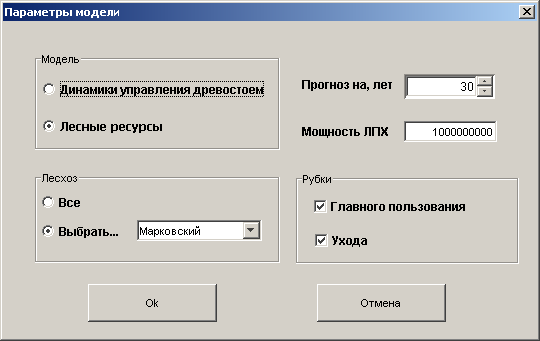
\includegraphics[width=405pt, height=256pt, keepaspectratio=true]{asyaDisser9_3-fig002.png}
\caption{Задание базовых параметров задачи}\label{pic:basic_task_params}
\end{figure}

Подсистема искусственного интеллекта позволяет автоматизировать процесс построения математической модели природного объекта на этапах идентификации параметров модели по исходным данным об объекте, синтеза структуры модели. В настоящее время база моделей информационной системы содержит модели ДУД и «Лесные ресурсы». Подсистема искусственного интеллекта реализована на основе базы знаний, содержащей знания о базовой структуре каждой модели, об идентификации модели на основе данных об исследуемом объекте, а также поиска начальных условий модели.

Исходные данные для идентификации модели и вычисления начальных условий загружаются из различных источников данных, которыми, как правило, выступают базы данных. Запросы к базам данных генерируются подпрограммами, запускаемыми механизмом логического вывода в процессе построения формализованного представления модели конкретного исследуемого объекта.

После импорта данных интерфейсным модулем программы производятся расчеты по модели, при этом предварительно выбирается один из вариантов стратегии управления лесными ресурсами (естественная или антропогенная динамика).

В режиме моделирования с использованием антропогенной динамики пользователь имеет возможность задавать управляющее воздействие (параметры рубок). Смена характера развития моделируемой природной системы отражается величиной коэффициентов модели, связанных со скоростью процессов возобновления и роста деревьев. Правила базы знаний позволяют гибко определять такие антропогенные воздействия на ЛР как объемы рубок, насаждений в зависимости от набора параметров. Например, объем рубок изменяется на каждом шаге интервала прогнозирования отдельно для каждого моделируемого участка, в зависимости от расчетных данных.

При расчетах по математическим моделям в той или иной мере используются пространственно-распределенные данные, что требует обеспечения тесного взаимодействия с современными ГИС, используемыми, в частности, для представления результатов прогнозных расчетов в виде цифровых карт. Автоматическое картографирование промежуточных стадий вычислений по моделям позволяет исследователю контролировать процесс моделирования.

\begin{center}
начало
База знаний

Ввод параметров задачи

Расчеты по модели

Многокритериальная оптимизация

Отображение данных расчетов

конецБаза данных

Идентификация модели

Формирование сценариев

Сохранение данных

Создание графиков

Создание карт, анимации

Рис. 3.4. Технологическая схема автоматизации
моделирования.
\end{center}

Комбинации значений параметров отображают управляющее воздействие на объект (гипотетическое решение ЛПР). В последнюю очередь определяются критерии\textit{ }анализа получаемых результатов прогнозных расчетов (расчета сценариев). Критерии свёртывают расчеты к набору числовых характеристик, которые идентифицируют сценарий и задают его положение в пространстве\textit{ }критериев. Заключительным этапом анализа модельных расчетов является многокритериальная оптимизация.

Полученные в результате расчета данные, например, в модели ДУД - распределение площадей по породам и классам возраста, а также и по времени, формируют базу данных формата CSV, и по запросу пользователя отображаются виде графиков, карт и  картографических анимаций (рис. 3.4).\label{HToc128995781}\label{HToc199746727}

\section{Информационное обеспечение системы}

Исходной информацией служат данные учета лесного фонда, которые представляют собой таблицы распределения площадей и запасов лесов по преобладающим породам и группам возраста. Основным источником информации о направлениях смены пород и возрастных циклах древостоев на всей территории лесхоза являются научные публикации, отражающие закономерности динамики леса в различных регионах. Эти обширные материалы составляют информационную основу подсистемы математического моделирования.

Данные для модели ДУД по Иркутской области содержат информацию по таким породам как сосна, ель, пихта, лиственница, кедр, береза, осина, а также в целом по хвойным и мягколиственным породам. В свою очередь они подразделяются на данные по группам возраста: молодняки 1, 2 класса и средневозрастные; приспевающие; спелые и перестойные. Также для расчетов используются данные о площади лесхоза, количестве населения, проживающего на территории лесхоза. Такие данные существуют по 53 из 59 лесхозов, имеющихся в Иркутской области.

Данные предоставлены Институтом географии СО РАН, по состоянию на 1 января 2004 г., по формам, утвержденным Рослехозом, в текстовых файлах формата *.txt. При передаче в информационную систему данные преобразованы в БД формата Microsoft Excel.

Эти данные используются для определения начальных и граничных условий решения дифференциальных уравнений модели ДУД, оценки комплексных характеристик состояния условий природной среды и вычисления ряда коэффициентов.

Для определения интенсивности рубок ухода и главного пользования использовались Правила рубок главного пользования в лесах Восточной Сибири [70] и Наставления по рубкам ухода в лесах Восточной Сибири [61]. Эти правила определяют порядок проведения рубок, их объемы, в зависимости от породы, класса возраста, распределения лесов по зонам и подзонам, крутизны склонов.

Данные для модели «Лесные ресурсы» находятся в БД поквартальных итогов. В материалах поквартальных итогов содержится информация о распределении площади квартала по категориям земель, площади и запасов лесов по породам и группам возраста, о средних таксационных характеристиках (табл. 1). В таблице 1 в столбце «Тип» значение «С» соответствует символьным данным, «Ц» - числовым.

{ \bf База знания была? Критерии были?}

\section{Результаты моделирования}

Информационная система поддержки принятия использована для расчета сценариев неистощительного использования ЛР Иркутской области. Получены несколько сценариев, в том числе без необходимости проводить лесовосстановительные мероприятия. Благодаря использованию базы знаний в качестве механизма построения и идентификации структуры и параметров модели процедура построения модели лесхозов Иркутской области оказалась достаточно простой не смотря на значительное огрубление исходных данных.

При построения модели лесхозов исходные данные включали только три класса возраста (молодняки I и II класса возраста, средневозрастные и приспевающие, спелые и перестойные), породы деревьев разделены также только на три класса (светлохвойные, темнохвойные и лиственные) без разделения по отдельным породам. При помощи уточнения набора правил построения модели ЛР Иркутской области создан новый набор правил построения и идентификации моделей ЛР по лесхозам. Проведенные расчеты также отображались в ГИС также в виде картографических произведений и анимации.

\section{Политика использования лесных ресурсов}

Разработанная в \cite{dissAsya} информационная систем поддержки принятия решений обладает возможностью анализировать потенциальные решения ЛПР, однако в ней предполагается, что данное решение остается неизменным за весь период моделирования, который, как правило, составляет 30, 50 или 100 лет. Однако политика использования лесных ресурсов претерпевает изменения: ЛПР в некоторый момент времени может повысить или понизить объемы рубок, увеличить и или уменьшить материальные затраты на борьбу с пожарами и вредителями. Логическое моделирование управления заготовкой ЛР на основе принятых ЛПР решений и их изменений во времени позволяет выработать более точный расчет режима использования ЛР.

(Про общую схему принятия решения ЛР, когда происходит выбор политики использования ЛР и на какой период)

\emph{Политикой использования лесного ресурса} (ПИЛР) будем называть набор правил, реализующих использование ЛР согласно некоторому решению ЛПР. Политика, будучи принятой, реализуется в виде заданного объема рубок, лесоустроительных мероприятий, а также мероприятиями по борьбе с пожарами и вредителями лесонасаждений. Задача логического моделирования состоит в том, чтобы выбрать и идентифицировать конкретную ПИЛР на очередной период времени.

(Про реальное и виртуальное время, как в лифтах)

Выбор и идентификация ПИЛР осуществляется следующим образом. В момент выбора ПИЛР в система порождает несколько альтернатив будущего, каждая альтернатива соответствует одному из возможных вариантов ПИЛР, в т.ч. ``сохранение прежнего курса''.

(Вот бы параметризировать ПИЛР на основе моделирования, как у ЛЕМПЕРТ: идентификация по серии экспериментов)


, точнее даже не правила и последовательность решений (логическая траектория), реализующий сценарий с заданным качеством. Но с другой стороны можно перемежать разные политика в смысле набора правил. Скажем каждые 5 лет принимается решение выбора политика на следующие пять лет, которые пять лет и выполняются. В этом случае получается, что база знаний становится еще богаче, а механизм моделирования становится еще богаче.

\emph{Логическое моделирование политики}

\subsection{Разновидности политик использования ЛР}
(Перечислить возможные политики)

\subsection{Организация принятия решения по выбору политики использования ЛР}

\section{Общие положения по использованию АДТ в синтезе и анализе .... (логических траекторий)}


(Разделение логической части, вычислительной и проверка ограничений. Предикаты с побочными действиями, вычислимые функции)

(Разделение )

\section{Логическая формализация задачи}

\subsection{Моделирование времени, temporal reasoning}
(Аксиома существования следующего момента времени)

\subsection{Ограничения на процесс поиска логического вывода}


\section{Примеры расчетов}


\section{Интерпретации результатов}

\section{Выводы по использованию АДТ}

... как механизма ПО-формул, как обеспечивающего ЛВ для всех 5 проблем: 1) temporal reasoning, 2) решения задачи без формализованной цели, 3) рассмотрение альтернативных вариантов решения ЛПР, 4) связь с вычислительными алгоритмами, 5) конструктивный вывод вперед с дизъюнкцией. 6) Обработка правилом вывода крупноблочных структур данных и большого количества атомов в конъюнкте базы.
